\documentclass[a4paper, 12pt]{article}

\usepackage{geometry}
\usepackage{amsmath}
\usepackage{gvv}

\title{Question 5.2.3}
\author{AI25BTECH11040 - Vivaan Parashar}
\date{\today}

\begin{document}

\maketitle

\section{Question: }
Solve the following system of linear equations:
\begin{align*}
    9x + 3y + 12 = 0\\
    18x + 6y + 24 = 0
\end{align*}

\section{Solution: }
The given equations can be rewritten as:
\begin{align}
    9x + 3y &= -12 \\
    18x + 6y &= -24
\end{align}
We can represent this system of equations in matrix form as:
\begin{align}
    \vec{M}\vec{X} = \vec{D}\\
    \implies \myvec{9 & 3 \\ 18 & 6} \myvec{x \\ y} = \myvec{-12 \\ -24}
\end{align}
To obtain values of $x$ and $y$, we can multiply both sides by the inverse of the coefficient matrix on the left side, but in this case, the coefficient matrix has a rank of 1 ($R_2 = 2R_1$). This implies that either the system has no solutions or infinite solutions.\\
If the system has infinite solution, then the rank of the augmented matrix $\myvec{\vec{M} & \vec{D}}$ should also have a rank of 1.
\begin{align}
    \rank(\myvec{\vec{M} & \vec{D}}) = \rank(\myvec{9 & 3 & -12 \\ 18 & 6 & -24})\\
    \myvec{9 & 3 & -12 \\ 18 & 6 & -24} \xleftrightarrow{R_2 = R_2 - 2R_1} \myvec{9 & 3 & -12 \\ 0 & 0 & 0}\\
    \therefore \rank(\myvec{\vec{M} & \vec{D}}) = 1
\end{align}
Therefore, this system of equations has infinite solutions, which are all values of $(x, y) \in \mathbb{R}^2$ that satisfy the equation $3x + y = -4$.\\

\section{Plot: }
\begin{figure}[h!]
    \centering
    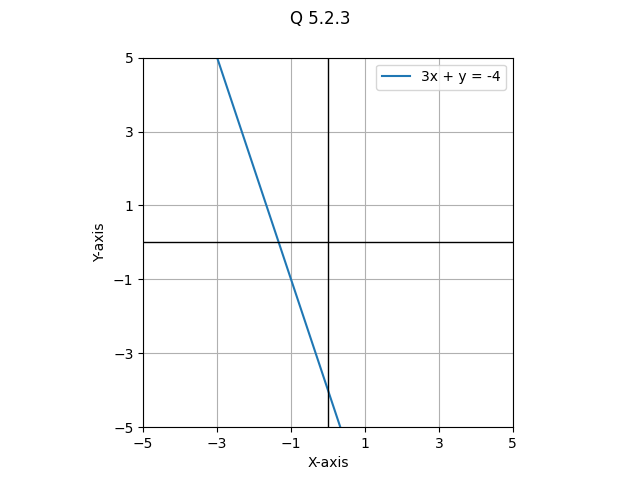
\includegraphics[width=\columnwidth]{figs/plot.png}
    \caption{Graph of line representing all possible solutions}
    \label{fig:5.2.3}
\end{figure}


\end{document}